\chapter{Introduction to molecular population genetics}

The study of evolutionary biology is commonly divided into two
components: study of the {\it processes\/} by which evolutionary
change occurs and study of the {\it patterns\/} produced by those
processes. By ``pattern'' we mean primarily the pattern of
phylogenetic relationships among species or genes.\footnote{In certain
  cases it may make sense to talk about a phylogeny of populations
  within species, but in many cases it doesn't. We'll discuss this
  further when we get to phylogeography in a couple of weeks.} Studies
of evolutionary processes often don't often devote too much attention
to evolutionary patterns, except insofar as it is often necessary to
take account of evolutionary history in determining whether or not a
particular feature is an adaptation. Similarly, studies of
evolutionary pattern sometimes try not to use any knowledge of
evolutionary processes to improve their guesses about phylogenetic
relationships, because the relationship between process and pattern
can be tenuous.\footnote{One way of justifying a strict parsimony
  approach to cladistics is by arguing (a) that by minimizing
  character state changes on a tree you're merely trying to find a
  pattern of character changes as consistent as possible with the data
  you've gathered and (b) that evolutionary processes should be
  invoked only to explain that pattern, not to construct it.} Those
who take this approach argue that invoking a particular evolutionary
process seems often to be a way of making sure that you get the
pattern you want to get from the data.\index{evolutionary pattern}\index{evolutionary process}

Or at least that's the way it was in evolutionary biology when
evolutionary biologists were concerned primarily with the evolution of
morphological, behavioral, and physiological traits and when
systematists used primarily anatomical, morphological, and chemical
features~(but not proteins or DNA) to describe evolutionary
patterns. With the advent of molecular biology after the Second World
War and its application to an increasing diversity of organisms in the
late 1950s and early 1960s, that began to
change. Goodman~\cite{Goodman62} used the degree of immunological
cross-reactivity between serum proteins as an indication of the
evolutionary distance among primates. Zuckerkandl and
Pauling~\cite{Zuckerkandl-Pauling65} proposed that after species
diverged, their proteins diverged according to a ``molecular clock,''
suggesting one that molecular similarities could be used to
reconstruct evolutionary history. In 1966, Harris~\cite{Harris66} and
Lewontin and Hubby~\cite{Hubby-Lewontin66,Lewontin-Hubby66} showed
that human populations and populations of {\it Drosophila
  pseudoobscura\/} respectively, contained surprising amounts of
genetic diversity.\index{molecular clock}\index{immunological distance}

In this course, we'll focus on advances made in understanding the
processes of molecular evolution and pay relatively little attention
to the ways in which inferences about evolutionary patterns can be
made from molecular data. Up to this point in the course we've
completely ignored evolutionary pattern. As you'll see in what
follows, however, any discussion of molecular evolution, even if it
focuses on understanding the processes, cannot avoid some careful
attention to the pattern.

\section*{Types of data}

Before we delve any further into our study of molecular evolution,
it's probably useful to back up a bit and talk a bit about the types
of data that are available to molecular evolutionists. We've already
encountered a couple of these (microsatellites and SNPs), but there
are a variety of important categories into which we can group data
used for molecular evolutionary analyses. Even though studies of
molecular evolution in the last 10-15 years have focused on data
derived from DNA sequence or copy number variation, modern
applications of molecular markers evolved from earlier
applications. Those markers had their limitations, but analyses of
them also laid the groundwork for most or all of what's going on in
analyses of molecular evolution today. Thus, it's useful to remind
everyone what those groups are and to agree on some terminology for
the ones we'll say something about. Let's talk first about the
physical basis of the underlying data. Then we'll talk about the
laboratory methods used to reveal variation.

\subsection*{The physical basis of molecular variation}

With the exception of RNA viruses, the hereditary information in all
organisms is carried in DNA. Ultimately, differences in any of the
molecular markers we study (and of genetically-based morphological,
behavioral, or physiological traits) is associated with some
difference in the physical structure of DNA, and molecular
evolutionists study a variety of its aspects.\index{molecular variation!physical basis}

\begin{description}

\item[Nucleotide sequence] A difference in nucleotide sequence is the
  most obvious way in which two homologous stretches of DNA may
  differ. The differences may be in translated portions of protein
  genes~(exons), portions of protein genes that are transcribed but
  not translated~(e.g., introns, 5' or 3' untranslated regions),
  non-transcribed functional regions~(e.g., promoters), or regions
  without apparent function.

\item[Protein sequence] Because of redundancy in the genetic code, a
  difference in nucleotide sequence at a protein-coding locus may or
  may not result in proteins with a different amino acid
  sequence. {\bf Important note}: Don't forget that some loci code for
  RNA that has an immediate function without being translated to a
  protein, e.g., ribosomal RNA and various small nuclear RNAs.

\item[Secondary, tertiary, and quaternary structure] Differences in
  amino acid sequence may or may not lead to a different distribution
  of $\alpha$-helices and $\beta$-sheets, to a different
  three-dimensional structure, or to different multisubunit
  combinations.

\item[Imprinting] At certain loci in some organisms the expression
  pattern of a particular allele depends on whether that allele was
  inherited from the individual's father or its mother.

\item[Expression] Functional differences among individuals may arise
  because of differences in the patterns of gene expression, even if
  there are no differences in the primary sequences of the genes that
  are expressed.\footnote{Of course, differences in expression must
    ultimately be the result of a DNA sequence~(or at least a
    methylation difference) difference somewhere, e.g., in a promoter
    sequence or the locus encoding a promotor or repressor protein, if
    it is a genetic difference or the result of an epigenetic
    modification of the sequence, e.g., by methylation.}

\item[Sequence organization] Particular genes may differ between
  organisms because of differences in the position and number of
  introns. At the whole genome level, there may be differences in the
  amount and kind of repetitive sequences, in the amount and type of
  sequences derived from transposable elements, in the relative
  proportion of G-C relative to A-T, or even in the identity and
  arrangement of genes that are present. In microbial species, only a
  subset of genes are present in all strains. For example, in {\it
    Streptococcus pneumoniae\/} the ``core genome'' contains only 73\%
  of the loci present in one fully sequenced reference
  strain~\cite{Obert-etal-2006}. Similarly, a survey of 20 strains of
  {\it Escherichia coli\/} and one of {\it E. fergusonii\/}, {\it
    E. coli\/}'s closest relative, identified only 2000 homologous
  loci that were present in all strains out of 18,000 orthologous loci
  identified~\cite{Touchon-etal-2009} 

\item[Copy number variation] Even within diploid genomes, there may be
  substantial differences in the number of copies of particular
  genes. In humans, for example, 76 copy-number polymorphisms (CNPs)
  were identified in a sample of only 20 individuals, and individuals
  differed from one another by an average of 11
  CNPs.~\cite{Sebat-etal-2004}.

\end{description}

\noindent It is worth remembering that in nearly all eukaryotes there
are two different genomes whose characteristics may be analyzed: the
nuclear genome and the mitochondrial genome. In plants there is a
third: the chloroplast genome. In some protists, there may be even
more, because of secondary or tertiary endosymbiosis. The
mitochondrial and chloroplast genomes are typically inherited only
through the maternal line, although some instances of biparental
inheritance are known.

\subsection*{Revealing molecular variation}

The diversity of laboratory techniques used to reveal molecular
variation is even greater than the diversity of underlying physical
structures. Various techniques involving direct measurement of aspects
of DNA sequence variation are by far the most common today, so I'll
mention only the techniques that have been most widely
used.\index{molecular variation!markers}

\begin{description}

\item[Immunological distance] Some molecules, notably protein
  molecules, induce an immune response in common laboratory
  mammals. The extent of cross-reactivity between an antigen raised to
  humans and chimps, for example, can be used as a measure of
  evolutionary distance. The immunological distance between humans and
  chimps is smaller than it is between humans and orangutans,
  suggesting that humans and chimps share a more recent common
  ancestor.

\item[DNA-DNA hybridization] Once repetitive sequences of DNA have
  been ``subtracted out'',\footnote{See below for a description of
    some of these repetitive seqeuences.} the rate and temperature at
  which DNA species from two different species anneal reflects the
  average percent sequence divergence between them. The percent
  sequence divergence can be used as a measure of evolutionary
  distance. Immunological distances and DNA-DNA hybridization were
  once widely used to identify phylogenetic relationships among
  species. Neither is now widely used in molecular evolution studies.

\item[Isozymes] Biochemists recognized in the late 1950s that many
  soluble enzymes occurred in multiple forms within a single
  individual. Population geneticists, notably Hubby and Lewontin, later
  recognized that in many cases, these different forms corresponded to
  different alleles at a single locus, {\it allozymes}. Allozymes are
  relatively easy to score in most macroscopic organisms, they are
  typically co-dominant (the allelic composition of heterozygotes can
  be inferred), and they allow investigators to identify both variable
  and non-variable loci.\footnote{Classical Mendelian genetics, and
    quantitative genetics too for that matter, depend on genetic
    variation in traits to identify the presence of a gene.} Patterns
  of variation at allozyme loci may not be representative of genetic
  variation that does not result from differences in protein structure
  or that are related to variation in proteins that are insoluble.

\item[RFLPs] In the 1970s molecular geneticists discovered restriction
  enzymes, enzymes that cleave DNA at specific 4, 5, or 6 base pair
  sequences, the {\it recognition site}. A single nucleotide change in
  a recognition site is usually enough to eliminate it. Thus, presence
  or absence of a restriction site at a particular position in a
  genome provides compelling evidence of an underlying difference in
  nucleotide sequence at that positon.

\item[RAPDs, AFLPs, ISSRs] With the advent of the polymerase chain
  reaction in the late 1980s, several related techniques for the rapid
  assessment of genetic variation in organisms for which little or no
  prior genetic information was available. These methods differ in
  details of how the laboratory procedures are performed, buty they
  are similar in that they (a) use PCR to amplify anonymous stretches
  of DNA, (b) generally produce larger amounts of variation than
  allozyme analyses of the same taxa, and (c) are bi-allelic, dominant
  markers. They have the advantage, relative to allozymes, that they
  sample more or less randomly through the genome. They have the
  disadvantage that heterozygotes cannot be distinguished from
  dominant homozygotes, meaning that it is difficult to use them to
  obtain information about levels of within population
  inbreeding.\footnote{To be fair, it is possible to distinguish
    heterozygotes from homozyotes with AFLPs, if you are {\it\bf
      very\/} careful with your PCR
    technique~\cite{Jansen-etal-2001}. That being said, few people are
    careful enough with their PCR to be able to score AFLPs reliably
    as codominant markers, and I am unaware of anyone who has done so
    outside of a controlled breeding program.}

\item[Microsatellites] Satellite DNA, highly repetitive DNA associated
  with heterochromatin, had been known since biochemists first began
  to characterize the large-scale structure of genomes in DNA-DNA
  hybridization studies. In the mid-late 1980s several investigators
  identified smaller repetitive units dispersed throughout many
  genomes. Microsatellites, which consist of short (2-6) nucleotide
  sequences repeated many times, have proven particularly useful for
  analyses of variation within populations since the
  mid-1990s. Because of high mutation rates at each locus, they
  commonly have many alleles. Moreover, they are typically
  co-dominant, making them more generally useful than dominant
  markers. Identifying variable microsatellite loci is more laborious
  than identifying AFLPs, RAPDs, or ISSRs.

\item[Nucleotide sequence] The advent of automated sequencing has
  greatly increased the amount of population-level data available on
  nucleotide sequences. Nucleotide sequence data has an important
  advantage over most of the types of data discussed so far:
  allozymes, RFLPs, AFLPs, RAPDs, and ISSRs may all hide
  variation. Nucleotide sequence differences need not be reflected in
  any of those markers. On the other hand, each of those markers
  provides information on variation at several or many, independently
  inherited loci. Nucleotide sequence information reveals differences
  at a location that rarely extends more than 2-3kb. Of course, as
  next generation sequencing techniques become less expensive and more
  widely available, we will see more and more examples of nucleotide
  sequence variation from many loci within individuals.

\item[Single nucleotide polymorphisms] In organisms that are
  genetically well-characterized it may be possible to identify a
  large number of single nucleotide positions that harbor
  polymorphisms. These SNPs potentially provide high-resolution
  insight into patterns of variation within the genome. For example,
  the HapMap project has identified approximately 3.2M SNPs in the
  human genome, or about one every kb~\cite{HapMap-2007}.

\end{description}

As you can see from these brief descriptions, each of the markers
reveals different aspects of underlying hereditary differences among
individuals, populations, or species. There is no single ``best''
marker for evolutionary analyses. Which is best depends on the
question you are asking. In many cases in molecular evolution, the
interest is intrinsically in the evolution of the molecule itself, so
the choice is based not on what those molecules reveal about the
organism that contains them but on what questions about which
molecules are the most interesting.

\section*{Divergence of nucleotide sequences}

Underlying much of what we're going to discuss in this last part of
the course is the idea that we should be able to describe the degree
of difference between nucleotide sequences, proteins, or anything else
as a result of some underlying evolutionary processes. To illustrate
the principle, let's start with nucleotide sequences and develop a
fairly simple model that describes how they become different over
time.\footnote{By now you should realize that when I write that
  somethin is ``fairly simple'', I mean that it's fairly simple to
  someone who's comfortable with mathematics.}\index{Jukes-Cantor distance}

Let $q_t$ be the probability that two homologous nucleotides are
identical after having been evolving for $t$ generations independently
since the gene in which they were found was replicated in their common
ancestor. Let $\lambda$ be the probability of a substitution occuring
at this nucleotide position in either of the two genes during a small
time interval, $\Delta t$. Then
\begin{eqnarray*}
q_{t+\Delta t} &=& (1 - \lambda\Delta t)^2q_t
                  + 2\left(1 - \lambda\Delta t\right)\left({1 \over
                           3}\lambda\Delta t\right)(1 - q_t)
                  + \hbox{o}(\Delta t^2) \\
               &=& (1 - 2\lambda\Delta t)q_t + \left({2 \over 3}\lambda
                                                    \Delta t\right)
                                              (1 - q_t) 
                  + \hbox{o}(\Delta t^2) \\
q_{t+\Delta t} - q_t &=& {2 \over 3}\lambda\Delta t - {8 \over
                           3}\lambda\Delta tq_t + \hbox{o}(\Delta t^2) \\
{q_{t+\Delta t} - q_t \over \Delta t} &=& {2 \over 3}\lambda - {8 \over
3}\lambda q_t + \hbox{o}(\Delta t) \\
\lim_{\Delta t\to 0}{q_{t+\Delta t} - q_t \over \Delta t}  = {dq_t \over dt} &=& {2 \over 3}\lambda - {8
\over 3}\lambda q_t \\
q_t &=& 1 - {3 \over 4}\left(1 - e^{-8\lambda t/3}\right) \\
\end{eqnarray*}
The expected number of nucleotide substitutions separating the two
sequences at any one position since they diverged is $d = 2\lambda
t$.\footnote{The factor 2 is there because $\lambda t$ substitutions
  are expected on each branch. In fact you will usually see the
  equation for $q_t$ written as $q_t = 1 - (3/4)\left(1 - e^{-4\alpha
      t/3}\right)$, where $\alpha = 2\lambda$. $\alpha$ is also
  referred to as the substitution rate, but it refers to the rate of
  substitution between the two sequences, not to the rate of
  substitution between each sequence and their common ancestor. If
  mutations are neutral $\lambda$ equals the mutation rate, while
  $\alpha$ equals twice the mutation rate.} Thus,
\begin{eqnarray*}
q_t &=& 1 - {3 \over 4}\left(1 - e^{-4d/3}\right) \\
d   &=& -{3 \over 4}\ln\left[1 - {4 \over 3}(1 - q_t)\right] \\
\end{eqnarray*}
This is the simplest model of nucleotide substitution
possible{\dash}the Jukes-Cantor model. It assumes\index{Jukes-Cantor distance!assumptions}

\begin{itemize}

\item that mutations are equally likely at all positions and

\item that mutation among all nucleotides is equally likely.

\end{itemize}

Let's examine the second of those assumptions first. Observed
differences between nucleotide sequences shows that some types of
substitutions, i.e., transitions~($A \iff G$, $T \iff C$), occur much
more frequently than others, i.e., transversions~($A \iff G$, $A \iff
C$, $T \iff A$, $T \iff G$). There are a variety of different
substitution models corresponding to different assumed patterns of
mutation: Kimura 2 parameter~(K2P), Felsenstein 1984~(F84),
Hasegawa-Kishino-Yano 1985~(HKY85), Tamura and Nei~(TrN), and
generalized time-reversible~(GTR). The GTR is, as its name suggests,
the most general {\it time-reversible\/} model. It allows substitution
rates to differ between each pair of nucleotides. That's why it's
general. It still requires, however, that the substitution rate be the
same in both directions. That's what it means to say that it's time
reversible. While it is possible to construct a model in which the
substitution rate differs depending on the direction of substitution,
it leads to something of a paradox: with non-reversible substitution
models the distance between two sequences $A$ and $B$ depends on
whether we measure the distance from $A$ to $B$ or from $B$ to~$A$.

There are two ways in which the rate of nucleotide substitution can be
allowed to vary from position to position{\dash}the phenomenon of
among-site rate variation. First, we expect the rate of substitution
to depend on codon position in protein-coding genes. The sequence can
be divided into first, second, and third codon positions and rates
calculated separately for each of those positions. Second, we can
assume {\it a priori\/} that there is a distribution of different
rates possible and that this distribution is described by one of the
standard distributions from probability theory. We then imagine that
the substitution rate at any given site is determined by a random draw
from the given probability distribution. The gamma distribution is
widely to describe the pattern of among-site rate variation, because
it can approximate a wide variety of different
distributions~(Figure~\ref{fig:asrv}).\footnote{And, to be honest,
  because it is mathematically convenient to work
  with.}\index{among-site rate variation}

\begin{figure}
\begin{center}
\resizebox{!}{8cm}{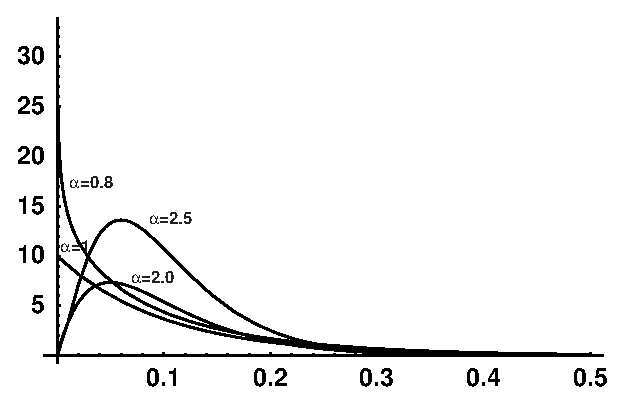
\includegraphics{gamma.eps}}
\end{center}
\caption{Examples of a gamma distribution.}\label{fig:asrv}
\end{figure}

The mean substitution rate in each curve above is 0.1. The curves
differ only in the value of a parameter, $\alpha$, called the ``shape
parameter.'' The shape parameter gives a nice numerical description of
how much rate variation there is, except that it's backwards. The
larger the parameter, the less among-site rate variation
there~is.\index{among-site rate variation!shape parameter}

